\section{Trigger Test of Trailing Lepton}

In $\mu\mu$ ($ee$) channel, at least one of leading and trailing leptons is 
required to pass single muon (electron) trigger test. Event is vetoed if 
both leading and trailing lepton fail to fire corresponding single lepton trigger.

In $e\mu$ channel, electron is required to fire single electron trigger and $p^T_e>p^T_\mu$.
In $\mu e$ channel, muon is required to fire single muon trigger and $p^T_\mu>p^T_e$.

Fig\ref{fig:triggerTest} shows the trailing $p^T$ in $\mu\mu$,$ee$,$\mu e$,$e\mu$.
In Fig\ref{fig:triggerTest}, data and MC events channel are split based on the trigger test of 
leading and trailing lepton.


\begin{figure}[h!]
  \centering
  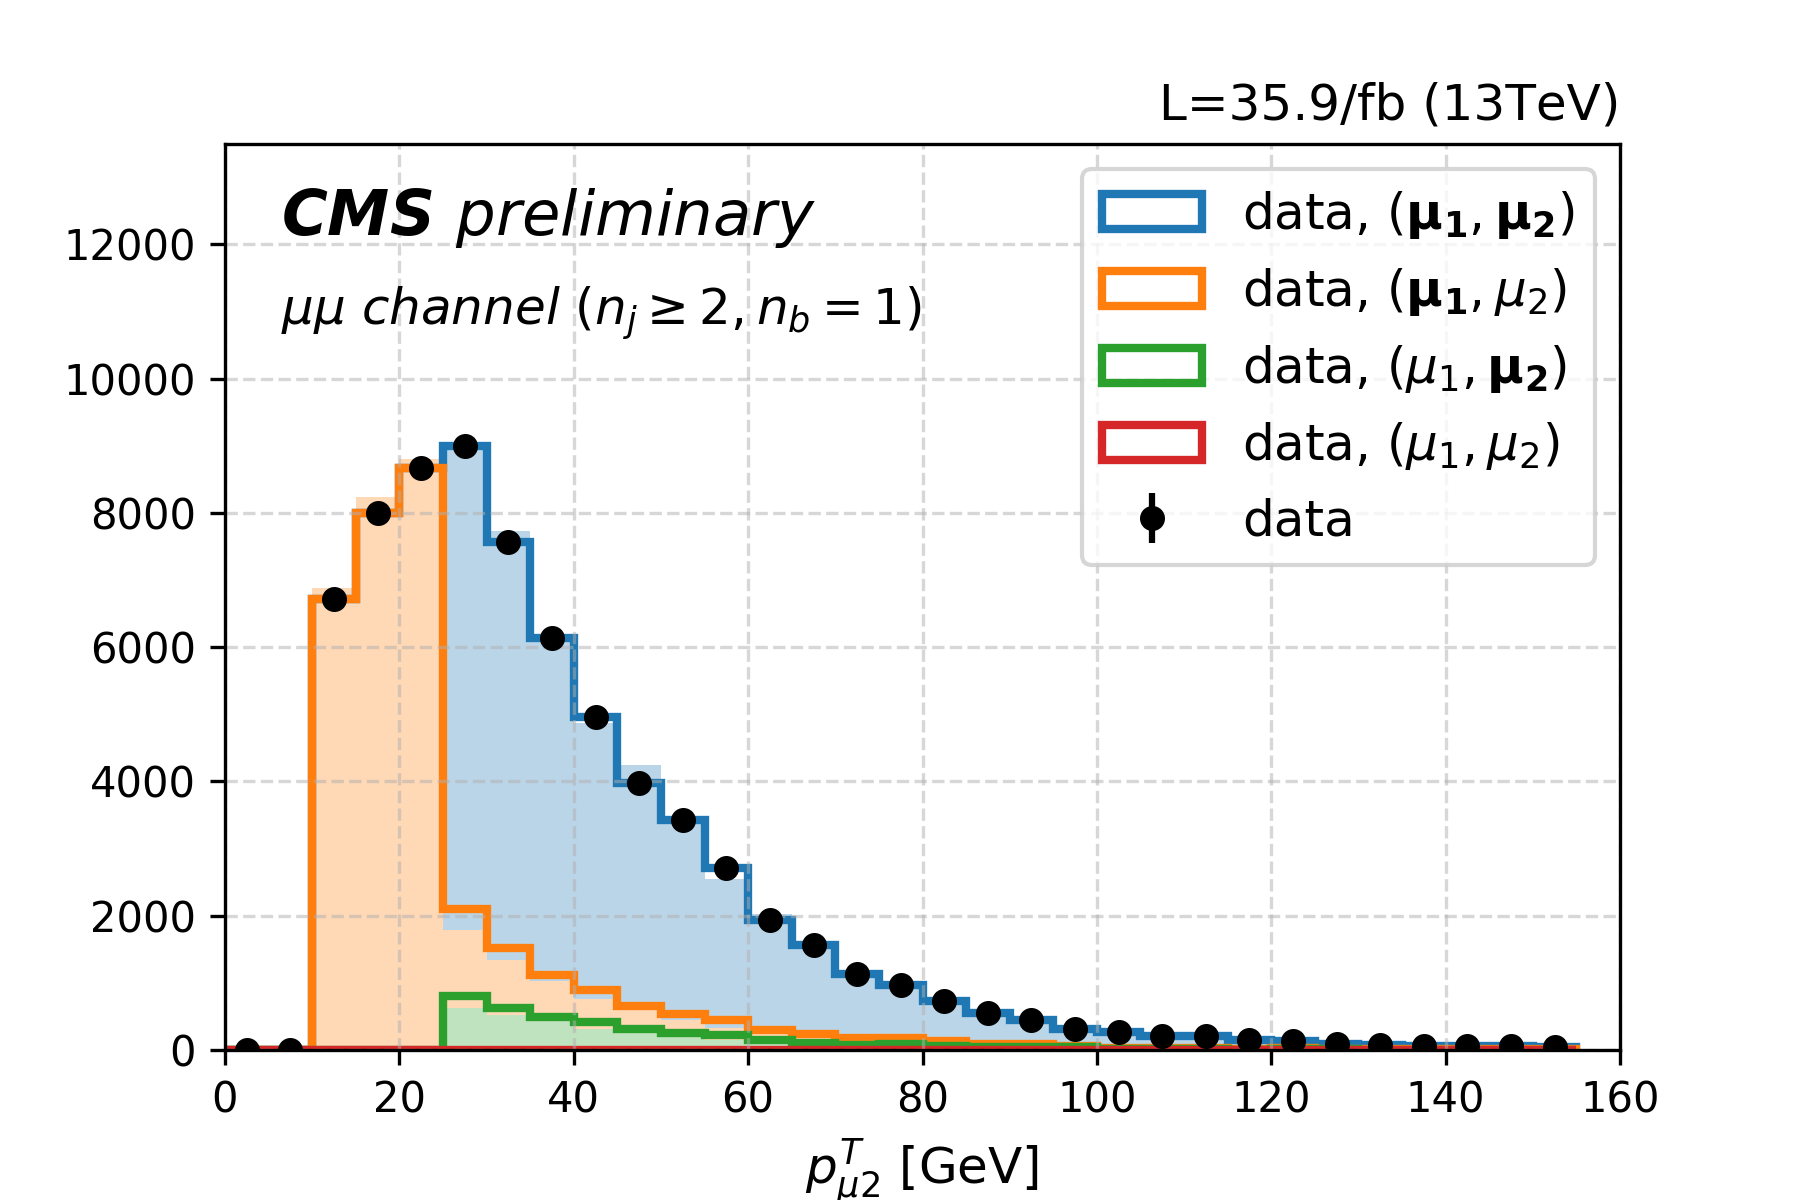
\includegraphics[width=0.49\textwidth]{chapters/Appendix/sectionTriggerTest/figures/trgLep_mumu.png}
  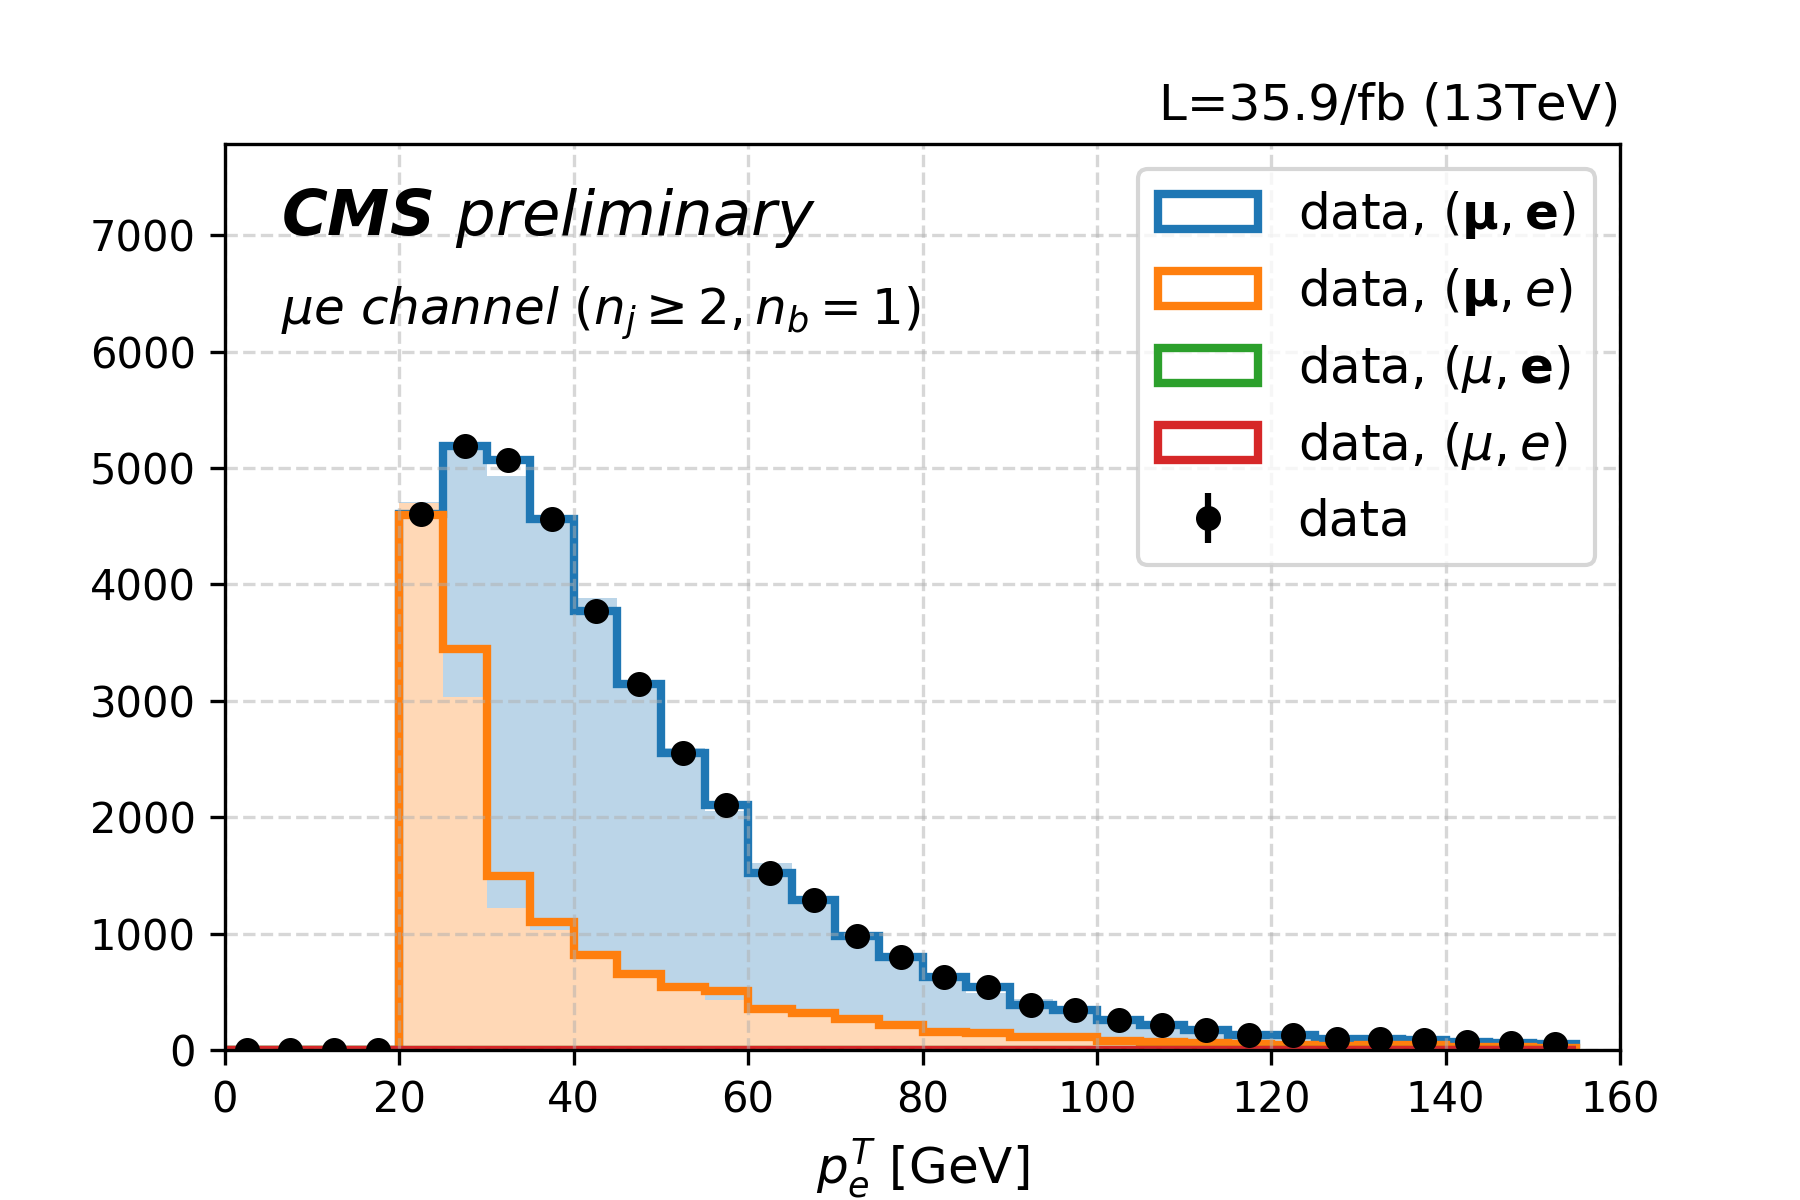
\includegraphics[width=0.49\textwidth]{chapters/Appendix/sectionTriggerTest/figures/trgLep_emu.png}
  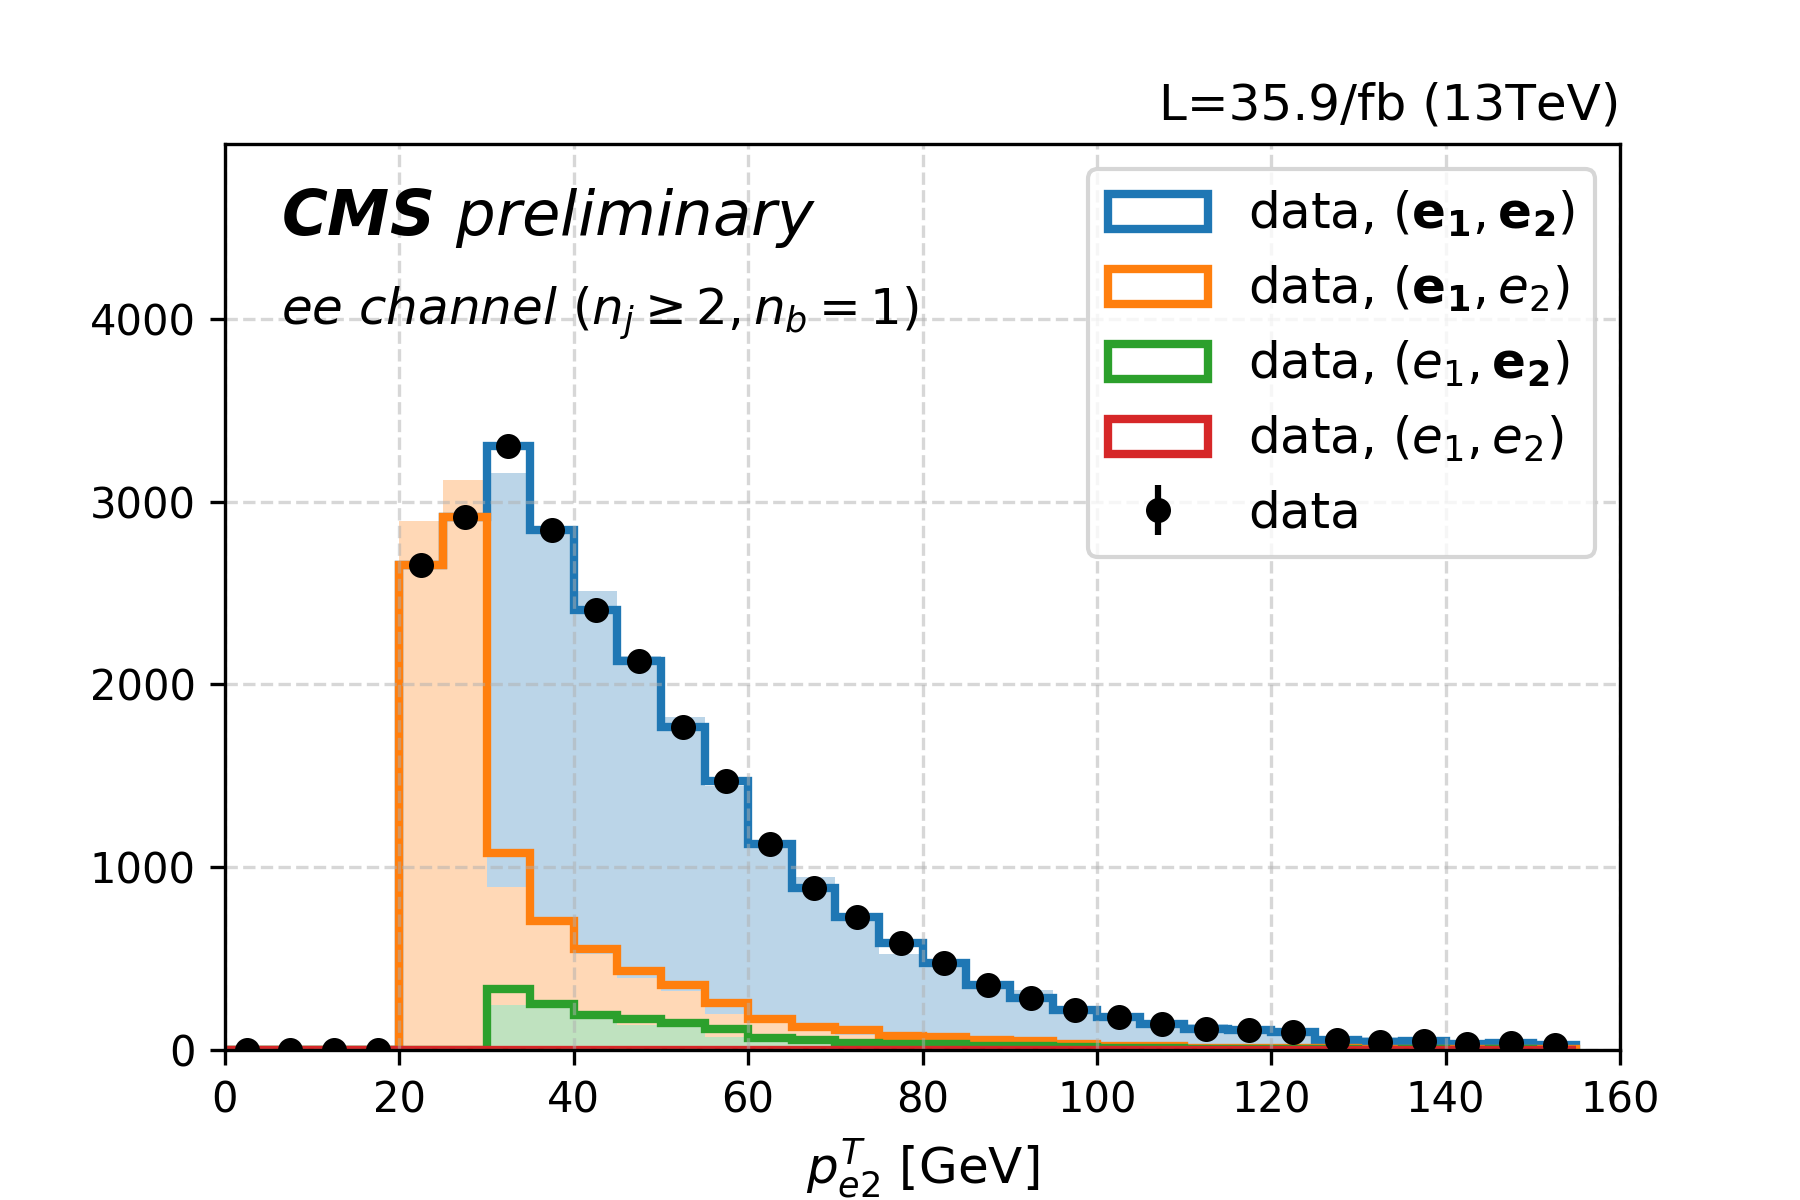
\includegraphics[width=0.49\textwidth]{chapters/Appendix/sectionTriggerTest/figures/trgLep_ee.png}
  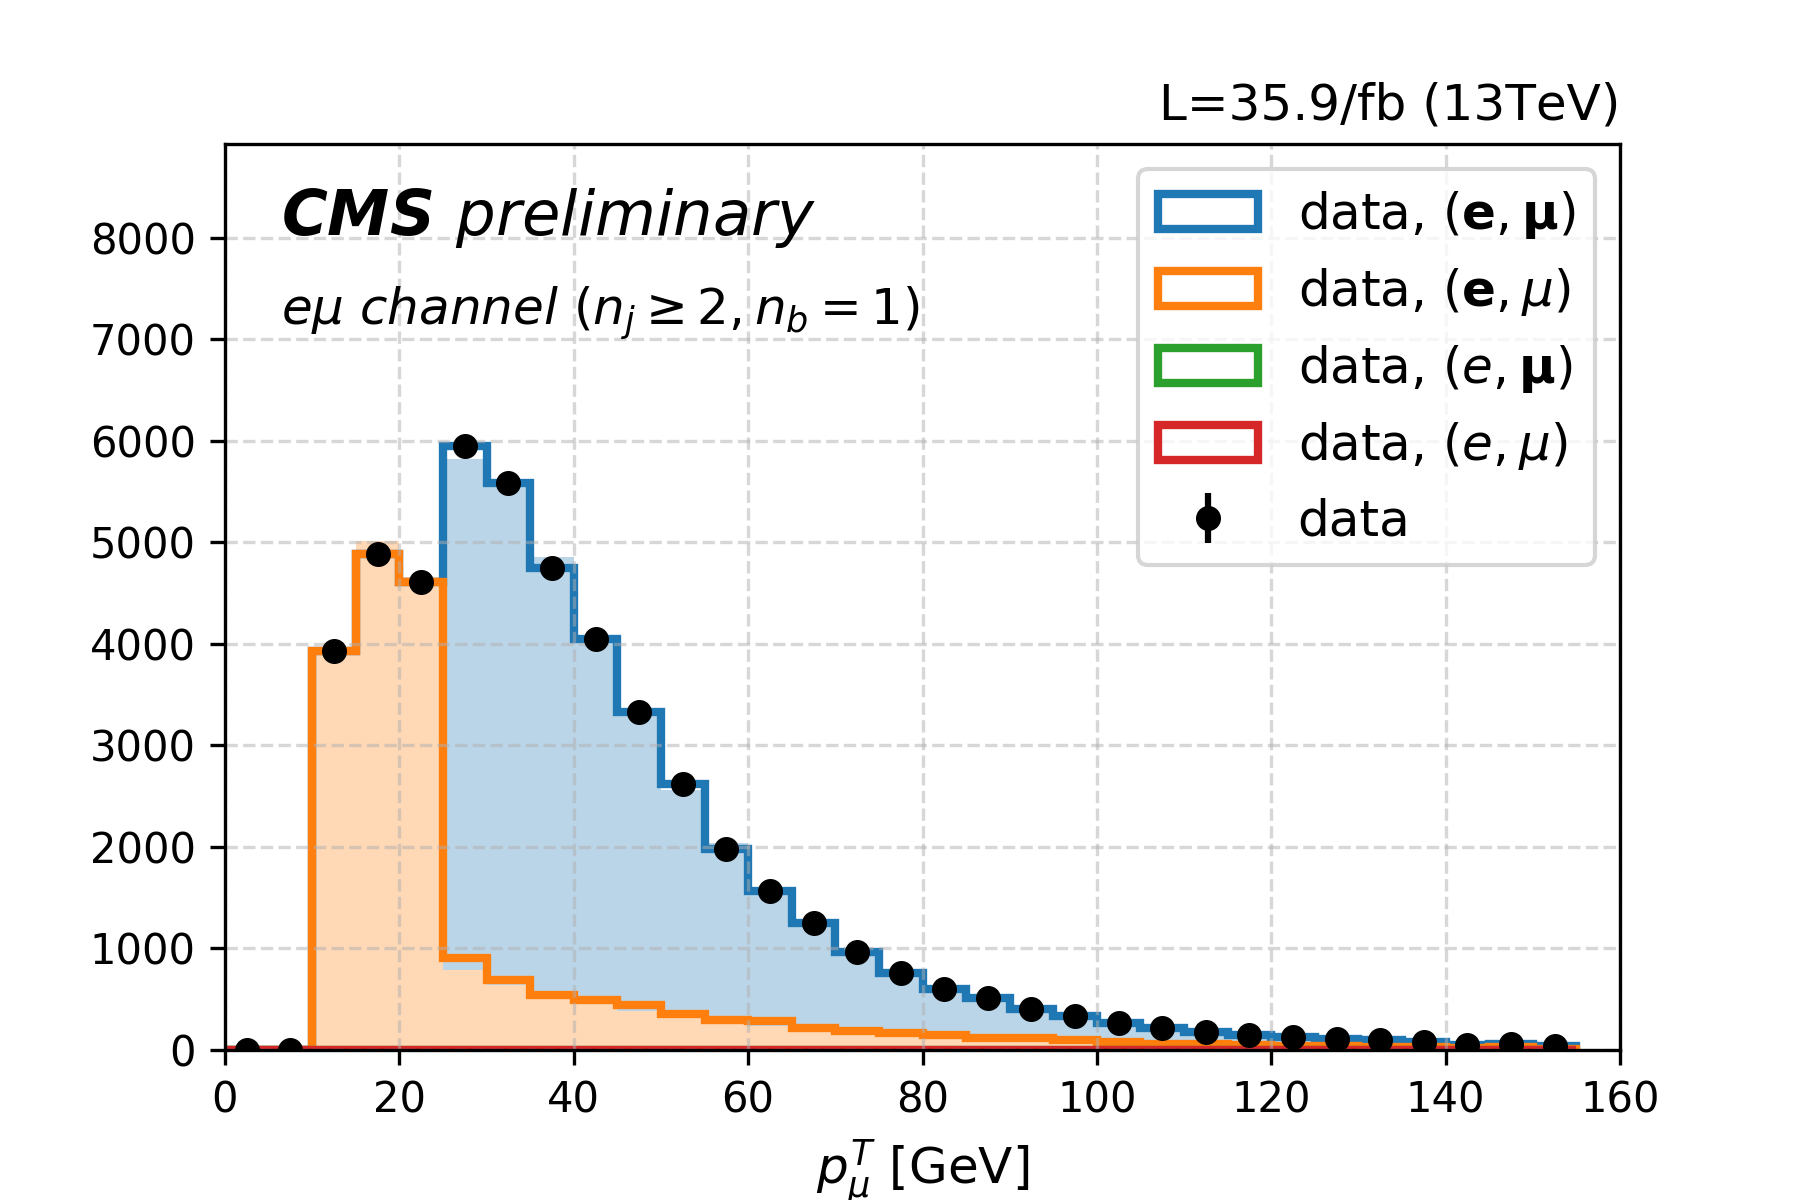
\includegraphics[width=0.49\textwidth]{chapters/Appendix/sectionTriggerTest/figures/trgLep_emu2.png}
  \caption{trailing $p^T$ in $\mu\mu$,$ee$,$\mu e$,$e\mu$. Data and MC events channel are split 
  based on the trigger test of leading and trailing lepton. 
  \label{fig:triggerTest}}
\end{figure}
\FloatBarrier